\documentclass[12pt]{article}

\usepackage{sbc-template}
\usepackage{graphicx,url}
\usepackage[utf8]{inputenc}
\usepackage[brazil]{babel}
\usepackage{booktabs}

\sloppy

\title{Análise Experimental do Tempo de Execução de Algoritmos de Ordenação:
  Quick Sort Recursivo, Quick Sort Iterativo e Merge Sort}

\author{Fernando Acácio Schatz\inst{1}, Yuri Oliveira di Golfeto\inst{1}}

\address{Departamento de Sistemas e Computação\\
  Universidade Regional de Blumenau (FURB) -- Blumenau -- SC -- Brasil}

\begin{document}

\maketitle

\section{Introdução}

Algoritmos de ordenação são componentes básicos de diversos sistemas, e a
escolha entre eles costuma ser feita a partir de análises teóricas de
complexidade. Este trabalho adota outra abordagem: compara, de forma
experimental, o tempo de execução de três algoritmos sobre a mesma entrada, em
um ambiente real de execução. Os algoritmos avaliados são o Quick Sort
Recursivo, o Quick Sort Iterativo e o Merge Sort~\cite{hoare1962,cormen2009}.

O objetivo é responder a quatro perguntas: (i) qual é o tempo médio de cada
algoritmo; (ii) quantas execuções são necessárias para estimar esse tempo com
erro relativo de 5\% e 95\% de confiança; (iii) se os intervalos de confiança
permitem distinguir os algoritmos; e (iv) se a ordem em que os algoritmos são
executados dentro de uma rodada altera os tempos medidos. Quando os intervalos
de confiança não são conclusivos, aplica-se a análise de variância (ANOVA)
seguida do teste de Tukey~\cite{montgomery2017,tukey1949}.

O código-fonte, os dados brutos em CSV e os scripts de análise estão no
repositório \url{https://github.com/FernandoAcacioSchatz/analise-de-algoritmo-trabalho-dois}.

\section{Metodologia}

\subsection{Ambiente e implementação}

Os algoritmos foram implementados em Python 3.13.13 (CPython), executados em
Windows 11 em um processador Intel (família 6, modelo 186). Os três
algoritmos seguem a mesma convenção: ordenam a lista recebida \emph{in-place} e
a devolvem.

O Quick Sort Recursivo e o Quick Sort Iterativo usam a mesma função de
partição, a partição de Lomuto com escolha do pivô pela mediana de três. A
única diferença entre eles é o controle de fluxo: o primeiro usa a pilha de
chamadas do interpretador, e o segundo usa uma pilha explícita de intervalos,
em que a maior subparte é empilhada primeiro. O Merge Sort é top-down, com um
único vetor auxiliar de tamanho $n$, alocado uma vez.

\subsection{Entrada}

A entrada é uma permutação aleatória dos inteiros de 0 a 99.999, ou seja, 100.000
valores distintos, gerada com a semente 42. A lista é gerada uma única vez,
salva em arquivo e lida a cada rodada, de modo que os três algoritmos recebem
exatamente a mesma sequência. Como os valores são distintos, o resultado
ordenado é conhecido e cada ordenação é verificada contra ele.

\subsection{Medição}

O tempo é medido com \texttt{time.perf\_counter\_ns()}. A cópia da entrada e a
verificação do resultado ficam fora da região cronometrada, e o coletor de lixo
do Python é desativado durante cada ordenação. Uma rodada executa os três
algoritmos em sequência, sobre cópias da mesma entrada.

\subsection{Rodízio}

Para evitar que a posição de execução se confunda com o algoritmo, as rodadas
seguem um rodízio completo: são usadas as seis ordens possíveis dos três
algoritmos (QR-QI-ME, QR-ME-QI, QI-QR-ME, QI-ME-QR, ME-QR-QI e ME-QI-QR), que
incluem as três rotações cíclicas. Assim, cada algoritmo ocupa cada posição em
duas ordens, e cada par de algoritmos aparece nas duas direções.

Antes da coleta, foram descartadas 18 rodadas de aquecimento, alternando as
seis ordens. Em seguida, uma amostragem piloto coletou 30 rodadas válidas por
formato.

\subsection{Número de execuções}

Para cada formato e cada algoritmo, calculou-se o menor $n$ que satisfaz

\begin{equation}
  n \geq \left(\frac{t_{\alpha/2,\,n-1}\cdot s}{E}\right)^2,
  \qquad E = 0{,}05\cdot\bar{x},
\end{equation}

em que $\bar{x}$ e $s$ são a média e o desvio padrão da amostra piloto e
$t_{\alpha/2,\,n-1}$ é o valor crítico de Student. O $n$ de cada formato é o
maior dos três valores, com piso de 30 rodadas. A coleta final prosseguiu,
alternando os formatos, até atingir o $n$ de cada um.

Como exemplo, considere o formato QR-QI-ME, cuja amostra piloto tem 30 rodadas
válidas por algoritmo. A Tabela~\ref{tab:calculo} mostra o cálculo para o Quick
Sort Recursivo (QR) e para o Merge Sort (ME). Como $t$ depende de $n$, testam-se
valores sucessivos até a condição ser satisfeita. Para o QR, $n = 24$ não
satisfaz, pois $(t\,s/E)^2 = 24{,}46 > 24$; $n = 25$ satisfaz, pois
$24{,}35 \leq 25$. Para o ME, $n = 66$ não satisfaz ($66{,}61 > 66$) e $n = 67$
satisfaz ($66{,}57 \leq 67$). Como o $n$ do formato é o maior dos três
algoritmos, o formato adota $n = 67$.

\begin{table}[ht]
\centering
\caption{Cálculo de $n$ no formato QR-QI-ME (amostra piloto de 30 rodadas).}
\label{tab:calculo}
\footnotesize
\begin{tabular}{lrrrrrr}
\toprule
Algoritmo & $\bar{x}$ (ms) & $s$ (ms) & $E$ (ms) & $s/E$ & $n$ & $(t\,s/E)^2$ \\
\midrule
QR & 98,43 & 11,77 & 4,92 & 2,391 & 25 & 24,35 \\
ME & 175,66 & 35,89 & 8,78 & 4,087 & 67 & 66,57 \\
\bottomrule
\end{tabular}
\end{table}

O enunciado indica ``5\% com 06\% de confiança'' em uma passagem e ``5\% com
95\% de confiança'' em outra. Adotou-se 95\%, que é o valor coerente com o
cálculo pedido.

\subsection{Análise estatística}

Para cada formato e algoritmo, calcularam-se a média, o desvio padrão e o
intervalo de confiança de 95\% da média, $\bar{x} \pm t_{\alpha/2,\,n-1}\,s/\sqrt{n}$.
Dois algoritmos com intervalos disjuntos são considerados diferentes. Quando
há sobreposição, aplica-se a ANOVA de um fator, com as premissas verificadas
pelo teste de Shapiro-Wilk (normalidade) e pelo teste de Levene (variâncias
homogêneas). Se a ANOVA for significativa, o teste de Tukey HSD identifica os
pares que diferem. O nível de significância é $\alpha = 0{,}05$.

\section{Resultados}

Foram realizadas 302 rodadas em 136 segundos, sendo 18 de aquecimento. Cada
algoritmo teve 284 rodadas válidas, distribuídas pelos formatos conforme o
cálculo de $n$. A Tabela~\ref{tab:medias} apresenta média e intervalo de
confiança de 95\% por formato e algoritmo. O erro relativo atingido ficou
abaixo de 5\% em todas as 18 combinações, com máximo de 4,81\%.

\begin{table}[ht]
\centering
\caption{Média e IC de 95\% (ms) do tempo de ordenação por formato.}
\label{tab:medias}
\footnotesize
\begin{tabular}{lrccc}
\toprule
Formato & $n$ & QR & QI & ME \\
\midrule
QR-QI-ME & 67 & 97,00 [94,81; 99,19] & 102,99 [100,43; 105,55] & 173,30 [167,14; 179,46] \\
QR-ME-QI & 91 & 97,47 [94,45; 100,50] & 103,49 [101,80; 105,18] & 170,74 [167,02; 174,46] \\
QI-QR-ME & 30 & 100,76 [97,36; 104,16] & 104,26 [100,96; 107,55] & 174,39 [170,89; 177,90] \\
QI-ME-QR & 36 & 101,01 [96,16; 105,87] & 107,32 [103,97; 110,68] & 173,24 [170,23; 176,25] \\
ME-QR-QI & 30 & 99,56 [96,12; 103,00] & 103,48 [100,16; 106,80] & 174,83 [169,36; 180,30] \\
ME-QI-QR & 30 & 96,66 [94,09; 99,23] & 104,13 [101,16; 107,11] & 170,29 [166,84; 173,73] \\
\bottomrule
\end{tabular}
\end{table}

\subsection{Comparação dos intervalos de confiança}

Em três formatos (QR-QI-ME, QR-ME-QI e ME-QI-QR) os intervalos dos três
algoritmos são disjuntos, e a comparação dos ICs é conclusiva: QR é
significativamente mais rápido que QI e ambos são mais rápidos que ME. Nos
formatos QI-QR-ME, QI-ME-QR e ME-QR-QI, os intervalos de QR e QI se sobrepõem.
Nesses três, o Merge Sort continua separado dos dois Quick Sorts, mas a
comparação entre QR e QI é inconclusiva. Por isso, aplicou-se o desafio extra
(ANOVA e Tukey) a esses três formatos.

\subsection{ANOVA e teste de Tukey}

A Tabela~\ref{tab:anova} resume os resultados nos três formatos inconclusivos.
A ANOVA é significativa em todos eles ($p < 0{,}001$), e o $\eta^2$ indica que o
algoritmo explica entre 90\% e 94\% da variação total dos tempos. O teste de
Tukey mostra que a diferença entre QR e QI não é significativa em nenhum dos
três formatos: os valores de $p$ ficam entre 0,051 e 0,371. Em QI-ME-QR, o
$p$ de 0,051 está no limite do nível de 5\%, e o intervalo da diferença quase
contém zero. Em todos os formatos, o Merge Sort difere dos dois Quick Sorts
($p < 0{,}001$).

\begin{table}[ht]
\centering
\caption{ANOVA de um fator e teste de Tukey nos formatos com ICs sobrepostos.}
\label{tab:anova}
\footnotesize
\begin{tabular}{lrrrrrl}
\toprule
Formato & $F$ & $\eta^2$ & Dif. QR$-$QI (ms) & $p$ Tukey & IC 95\% da dif. \\
\midrule
QI-QR-ME & 624,82 & 0,935 & $-3{,}50$ & 0,302 & $[-9{,}10;\ 2{,}11]$ \\
QI-ME-QR & 450,91 & 0,896 & $-6{,}31$ & 0,051 & $[-12{,}65;\ 0{,}02]$ \\
ME-QR-QI & 426,73 & 0,907 & $-3{,}92$ & 0,371 & $[-10{,}84;\ 3{,}00]$ \\
\bottomrule
\end{tabular}
\end{table}

\subsection{Premissas}

As variâncias foram homogêneas nos três formatos (teste de Levene, $p$ entre
0,07 e 0,96). O teste de Shapiro-Wilk rejeitou a normalidade em pelo menos um
algoritmo de cada formato, e em um deles para todos os algoritmos. Como cada
grupo tem entre 30 e 36 rodadas, a ANOVA e o teste de Tukey são considerados
robustos a esse desvio, mas isso fica registrado como limitação.

\subsection{Efeito da ordem de execução}

Nas Figuras~\ref{fig:fmt} e~\ref{fig:alg} observa-se a série de tempos ao
longo das rodadas. A média de cada algoritmo varia de um formato para outro
por cerca de 4 a 5 ms. Essa variação é da mesma ordem de grandeza da largura
dos intervalos de confiança, e não foi testada formalmente como efeito de
posição. Picos isolados de tempo ocorrem em trechos específicos da coleta,
como nas rodadas 90 a 110, e afetam os três algoritmos.

\begin{figure}[ht]
\centering
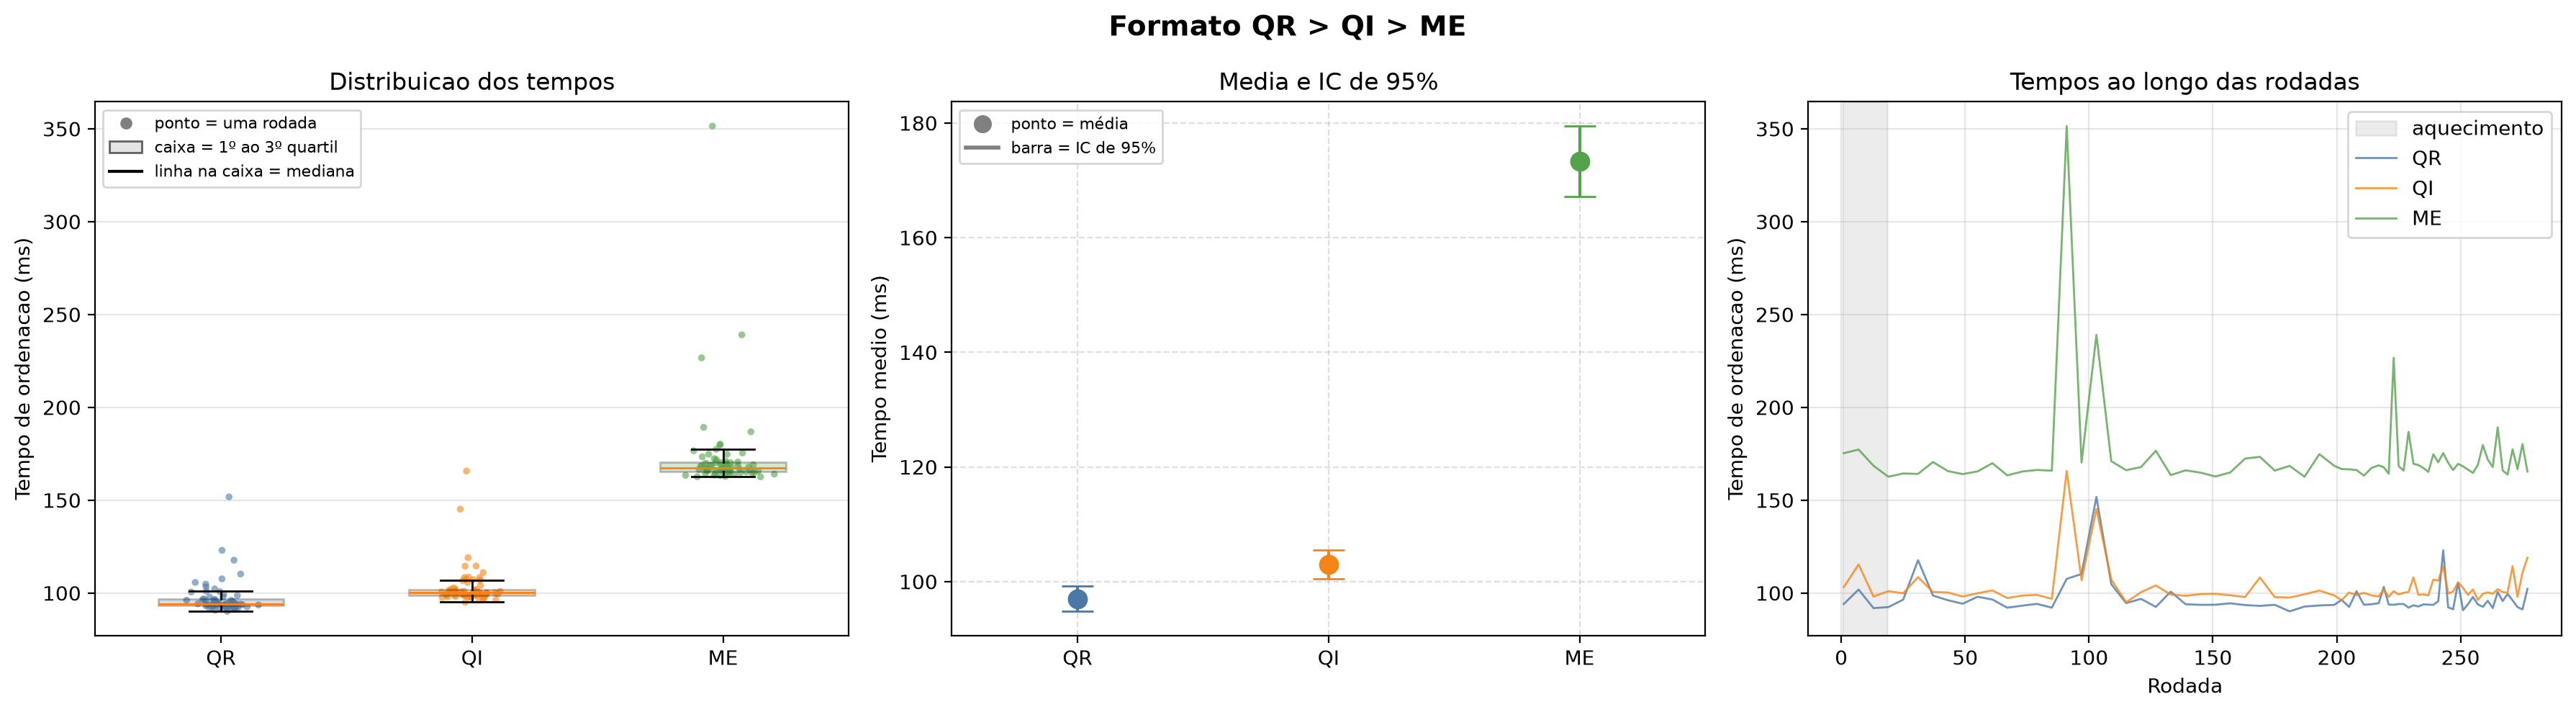
\includegraphics[width=\linewidth]{figuras/fmt_QR-QI-ME.png}
\caption{Formato QR-QI-ME: distribuição, média com IC de 95\% e tempo de
  cada rodada.}
\label{fig:fmt}
\end{figure}

\begin{figure}[ht]
\centering
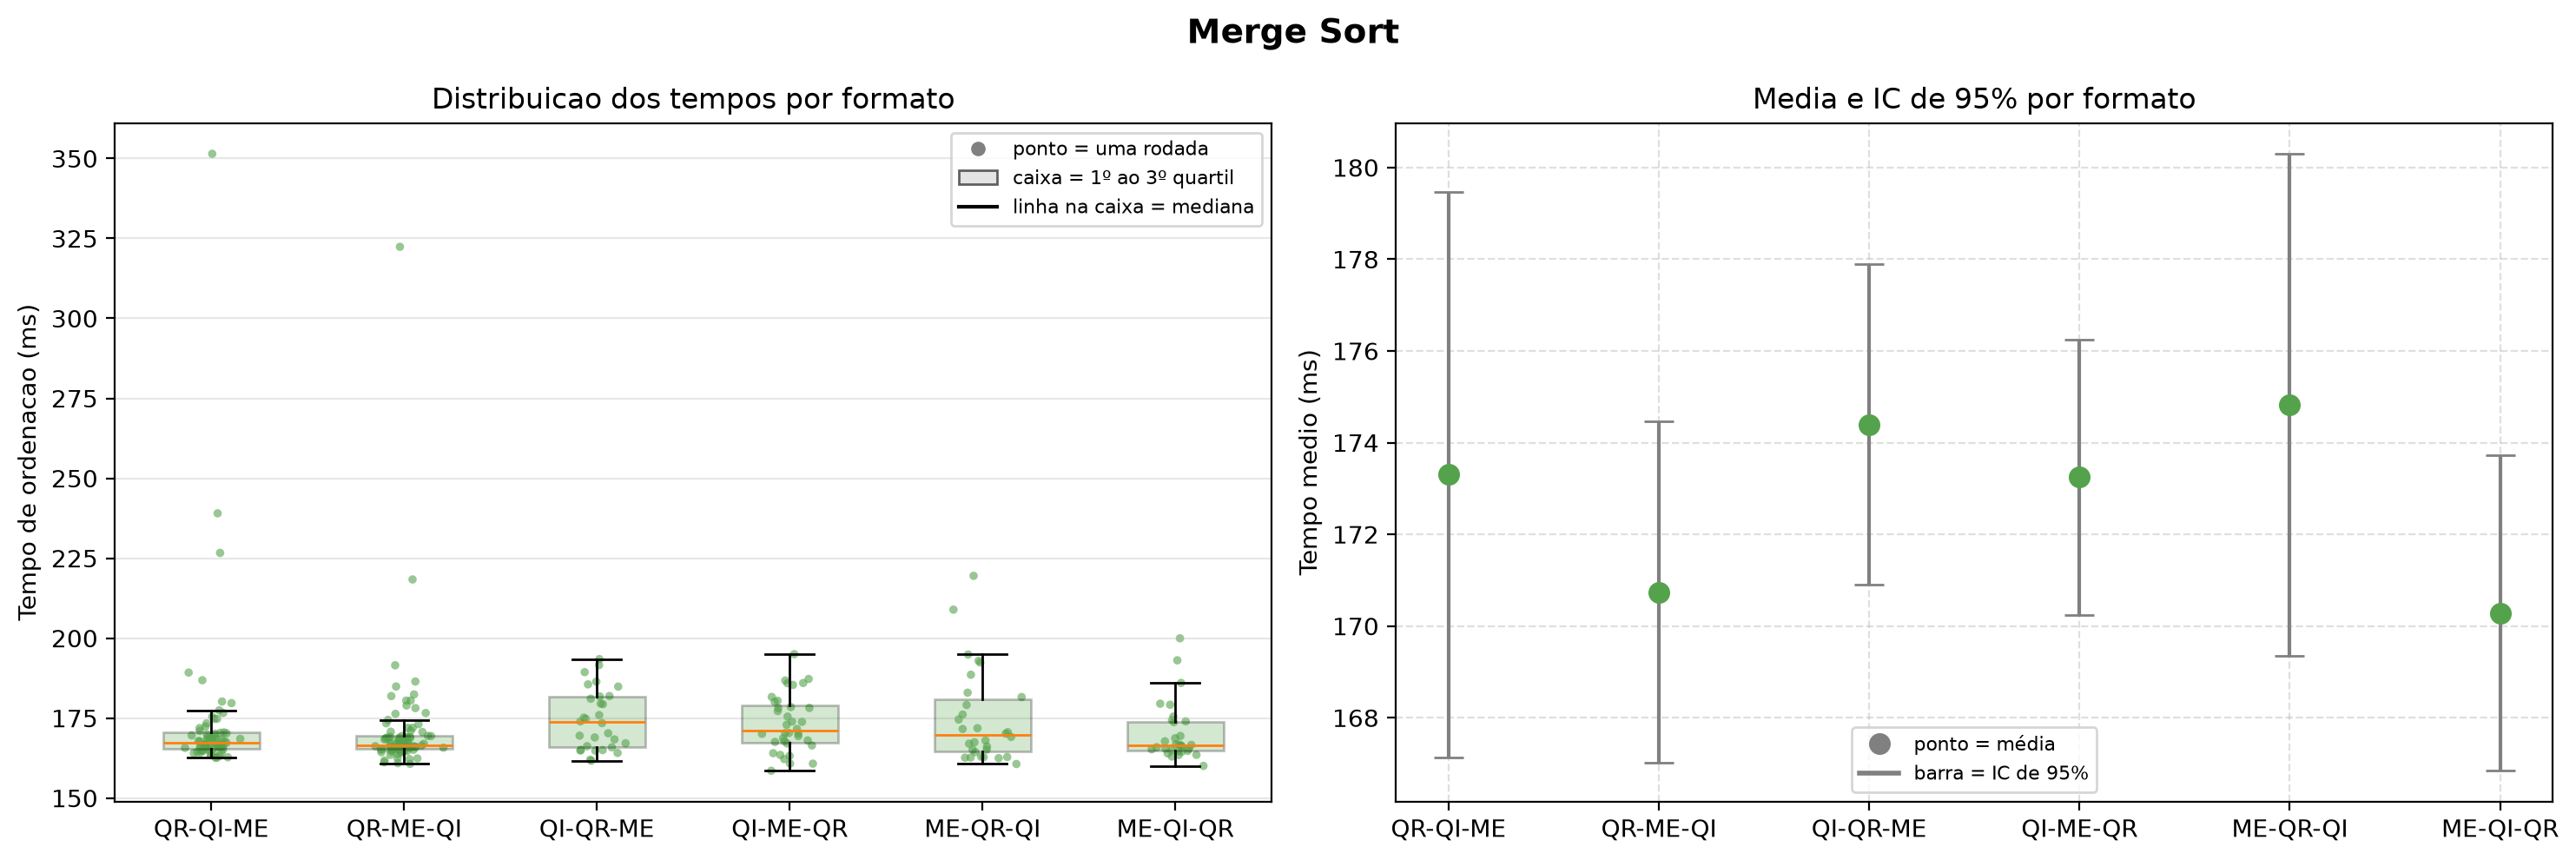
\includegraphics[width=\linewidth]{figuras/alg_Merge_Sort.png}
\caption{Merge Sort nos seis formatos.}
\label{fig:alg}
\end{figure}

\section{Discussão}

Com base nos experimentos, o Merge Sort foi o mais lento em todos os formatos.
Sua média global é de 172,8 ms, contra 98,7 ms do Quick Sort Recursivo e
104,3 ms do Quick Sort Iterativo, ou seja, cerca de 74 ms a mais que o
recursivo. Esse resultado é estável: o intervalo do Merge Sort nunca se
sobrepõe ao dos dois Quick Sorts. Uma explicação plausível é o custo de copiar
os dados para o vetor auxiliar em cada nível da recursão, enquanto os Quick
Sorts trocam elementos no próprio vetor. Essa explicação é uma hipótese e não
foi testada diretamente.

Entre os dois Quick Sorts, o recursivo foi o mais rápido na média, com uma
diferença de cerca de 5,5 ms (aproximadamente 5\%). A diferença é
estatisticamente clara em três formatos, pelos intervalos disjuntos, e não é
detectada pelo Tukey nos outros três. Portanto, a conclusão mais forte que os
dados permitem é que o Quick Sort Recursivo é o algoritmo mais rápido nesta
configuração, mas com vantagem pequena sobre o Iterativo. Como os dois usam a
mesma partição, a diferença vem apenas do controle de fluxo, e a pilha
explícita em Python pode custar um pouco mais que a recursão. Essa também é
uma hipótese.

As limitações do estudo são as seguintes. Todos os experimentos foram feitos
em uma única máquina, com Python, em um único tamanho de entrada e em uma
única distribuição (permutações de inteiros distintos). Os tempos dependem do
ambiente: durante a coleta o navegador Microsoft Edge estava aberto, e há
picos de tempo em trechos específicos da série. Os resultados não devem ser
extrapolados para implementações em linguagens compiladas nem para entradas
com muitos valores repetidos.

\section{Conclusão}

Nas condições testadas, o Merge Sort é claramente mais lento que os dois Quick
Sorts, com diferença de cerca de 75\%. O Quick Sort Recursivo apresentou a
menor média global, mas sua vantagem sobre o Quick Sort Iterativo é pequena e
só é estatisticamente clara em parte dos formatos. A ordem de execução dentro
da rodada não produziu mudanças sistemáticas acima da variação já observada,
e o rodízio completo permitiu verificar isso.

\bibliographystyle{sbc}
\bibliography{refs}

\end{document}
